% APLAS 2024: Regular research papers should not exceed 17 pages in
% the Springer LNCS format(LaTeX template), including bibliography and
% figures.
% Lightweight double-blind: Author names and institutions must be
% omitted and References to the authors’ own related work should be in
% the third person 
%
\documentclass[runningheads]{llncs}
\pdfoutput=1
\usepackage[utf8]{inputenc}
\usepackage{amsmath}
\usepackage{amssymb}
\usepackage{graphicx}
\usepackage{mathpartir}
\usepackage{xcolor}
\usepackage{hyperref}
\usepackage{listings}

\lstdefinelanguage{michelson}{
  basicstyle=\ttfamily,
  basicstyle=\fontsize{8}{9.6}\selectfont,
  morekeywords={parameter,storage,or,unit,mutez,pair,bool,address}, sensitive=false,
  morecomment=[l]{\#},
  morecomment=[s]{/*}{*/},
  morestring=[b]",
}

%% structure
\newcommand{\Angle}[1]{\langle#1\rangle}

%% values
\newcommand{\NEG}{\neg}
\newcommand{\CNF}{\wedge}
\newcommand{\DNF}{\vee}
\newcommand{\TRUE}{\text{True}}
\newcommand{\FALSE}{\text{False}}
\newcommand{\EMPTYSTRING}{\text{$""$}}
\newcommand{\STACKCONCAT}{\text{$::$}}
\newcommand{\ZERO}{\text{0}}
\newcommand{\ONE}{\text{1}}
\newcommand{\VAMOUNT}{\text{amount}}
\newcommand{\VCONTRACT}{\text{contract}}

%% contract constants
\newcommand{\CAMOUNT}{\text{amount}}
\newcommand{\CBALANCE}{\text{balance}}
\newcommand{\CSENDER}{\text{sender}}
\newcommand{\CSOURCE}{\text{source}}
\newcommand{\CNOW}{\text{now}}
\newcommand{\CLEVEL}{\text{level}}
\newcommand{\CCHAINID}{\text{chain-id}}
\newcommand{\CSELF}{\text{self}}
\newcommand{\CSELFADDRESS}{\text{self-address}}
\newcommand{\CTOTALVOTINGPOWER}{\text{total-voting-power}}
\newcommand{\CVOTINGPOWER}{\text{voting-power}}

%% contract instructions
\newcommand{\AMOUNT}{\text{AMOUNT}}
\newcommand{\BALANCE}{\text{BALANCE}}
\newcommand{\SENDER}{\text{SENDER}}
\newcommand{\SOURCE}{\text{SOURCE}}
\newcommand{\NOW}{\text{NOW}}
\newcommand{\LEVEL}{\text{LEVEL}}
\newcommand{\CHAINID}{\text{CHAIN-ID}}
\newcommand{\SELF}{\text{SELF}}
\newcommand{\SELFADDRESS}{\text{SELF-ADDRESS}}
\newcommand{\TOTALVOTINGPOWER}{\text{TOTAL-VOTING-POWER}}
\newcommand{\VOTINGPOWER}{\text{VOTING-POWER}}
\newcommand{\MinusBalanceAmount}{\text{BALANCE-AMOUNT}}
%% auction contract
\newcommand{\AuctionOwner}{\text{auction-owner}}
\newcommand{\AuctionBidder}{\text{auction-bidder}}
\newcommand{\AuctionClose}{\text{auction-close}}
\newcommand{\AuctionOpen}{\text{auction-open}}
\newcommand{\AuctionBid}{\text{auction-bid}}

%% system definition
\newcommand{\VAL}{\textbf{v}}
\newcommand{\VAR}{\textbf{x}}
\newcommand{\VARIABLE}{\text{$Var$}}
\newcommand{\CONSTANT}{\text{$Const$}}
\newcommand{\TERM}{\text{$T$}}
\newcommand{\VariableX}{\text{$x$}}
\newcommand{\VariableV}{\text{$v$}}
\newcommand{\VariableK}{\text{$k$}}
\newcommand{\VariableA}{\text{$a$}}
\newcommand{\VariableB}{\text{$b$}}
\newcommand{\ELT}{\text{$Elt$}}
\newcommand{\A}{\text{$A$}}
\newcommand{\B}{\text{$B$}}
\newcommand{\N}{\text{$n$}}
\newcommand{\K}{\text{$k$}}
\newcommand{\V}{\text{$v$}}
\newcommand{\M}{\text{$m$}}
\newcommand{\VariableOne}{\text{$x_1$}}
\newcommand{\VariableTwo}{\text{$x_2$}}
\newcommand{\VariableN}{\text{$x_n$}}
\newcommand{\Constant}{\text{$c$}}
\newcommand{\ConstantOne}{\text{$c_1$}}
\newcommand{\ConstantTwo}{\text{$c_2$}}
\newcommand{\ConstantN}{\text{$c_n$}}
\newcommand{\LIST}{\text{$l$}}
\newcommand{\EMPTYLIST}{\text{$\{\}$}}
\newcommand{\TLIST}{\text{$l'$}}
\newcommand{\HEAD}{\text{$hd$}}
\newcommand{\TAIL}{\text{$tl$}}
\newcommand{\STAIL}{\text{$< tl >$}}
\newcommand{\Term}{\text{$t$}}
\newcommand{\TermOne}{\text{$t_1$}}
\newcommand{\TermTwo}{\text{$t_2$}}
\newcommand{\TermN}{\text{$t_n$}}
\newcommand{\TermB}{\text{$t_b$}}
\newcommand{\STACK}{\text{$S$}}
\newcommand{\EMPTYSTACK}{\text{[ ]}}
\newcommand{\STACKONE}{\text{$S$}}
\newcommand{\STACKTWO}{\text{$S$}}
\newcommand{\STACKN}{\text{$S$}}
\newcommand{\Stack}{\text{$s$}}
\newcommand{\StackOne}{\text{$s_1$}}
\newcommand{\StackTwo}{\text{$s_2$}}
\newcommand{\StackN}{\text{$s_n$}}
\newcommand{\TSTACK}{\text{$S'$}}
\newcommand{\TStack}{\text{$s'$}}
\newcommand{\STATE}{\text{$ST$}}
\newcommand{\STATEONE}{\text{$ST_1$}}
\newcommand{\STATETWO}{\text{$ST_2$}}
\newcommand{\STATEN}{\text{$ST_n$}}
\newcommand{\SYSTEM}{\text{$SE$}}
\newcommand{\INSTRUCTION}{\text{$I$}}
\newcommand{\TINSTRUCTION}{\text{$I'$}}
\newcommand{\INSTRUCTIONONE}{\text{$I1$}}
\newcommand{\INSTRUCTIONTWO}{\text{$I2$}}
\newcommand{\Instruction}{\text{$i$}}
\newcommand{\TInstruction}{\text{$i'$}}
\newcommand{\InstructionOne}{\text{$i_1$}}
\newcommand{\InstructionTwo}{\text{$i_2$}}
\newcommand{\InstructionN}{\text{$i_n$}}
\newcommand{\Invariant}{\text{$Iv$}}
\newcommand{\PREDICATE}{\text{$P$}}
\newcommand{\PREDICATEA}{\text{$P_A$}}
\newcommand{\PREDICATEB}{\text{$P_B$}}
\newcommand{\Predicate}{\text{$p$}}
\newcommand{\Failwith}{\text{$Failwith$}}
\newcommand{\PredicateOne}{\text{$p_1$}}
\newcommand{\PredicateTwo}{\text{$p_2$}}
\newcommand{\PredicateN}{\text{$p_n$}}
\newcommand{\SETA}{\text{$\mathcal{A}$}}
\newcommand{\SETAAUCTION}{\text{$\mathcal{A}_{auction}$}}
\newcommand{\SETPOST}{\text{$\mathcal{A'}$}}
\newcommand{\SETPOSTAUCTION}{\text{$\mathcal{A'}_{auction}$}}
\newcommand{\EMPTY}{\text{$\O$}}
\newcommand{\PCreate}{\text{$P_{Create}$}}
\newcommand{\PBidding}{\text{$P_{Bidding}$}}
\newcommand{\PClose}{\text{$P_{Close}$}}
\newcommand{\SE}{\text{SE}}
\newcommand{\SINIT}{\text{$s_{init}$}}
\newcommand{\SFINAL}{\text{$s_{final}$}}
\newcommand{\FMAP}{\textbf{map}}
\newcommand{\MAPA}{\textbf{$map_A$}}
\newcommand{\MAPB}{\textbf{$map_B$}}
\newcommand{\MapBidding}{\textbf{$map_{bidding}$}}
\newcommand{\MapCreate}{\textbf{$map_{create}$}}
\newcommand{\MapClose}{\textbf{$map_{close}$}}
\newcommand{\MAPER}{\text{$\overline{\textbf{map}}$}}


%% operation
\newcommand{\CONS}{\text{cons}}
\newcommand{\NIL}{\text{nil}}
\newcommand{\PLUS}{\textbf{+}}
\newcommand{\MINUS}{\textbf{-}}
\newcommand{\EQUAL}{\textbf{=}}
\newcommand{\LESS}{\textbf{$<$}}
\newcommand{\LESSEQUAL}{\textbf{$<=$}}
\newcommand{\MORE}{\textbf{$>$}}
\newcommand{\MOREEQUAL}{\textbf{$>=$}}

%% instructions
\newcommand{\UNIT}{\text{Unit}}
\newcommand{\PAIR}{\text{Pair}}
\newcommand{\LEFT}{\text{Left}}
\newcommand{\RIGHT}{\text{Right}}
\newcommand{\SOME}{\text{Some}}
\newcommand{\NONE}{\text{None}}
\newcommand{\ADD}{\text{ADD}}
\newcommand{\DROP}{\text{DROP}}
\newcommand{\LOOP}{\text{LOOP}}
\newcommand{\FAILWITH}{\text{FAILWITH}}
\newcommand{\TRANSFER}[2]{\text{Transfer($#1$, $#2$)}}
\newcommand{\CONTRACT}{\text{CONTRACT}}
\newcommand{\CAR}{\text{CAR}}
\newcommand{\EXEC}{\text{EXEC}}
\newcommand{\APPLY}{\text{APPLY}}
\newcommand{\IF}{\text{IF}}
\newcommand{\IFLEFT}{\text{IF-LEFT}}
\newcommand{\IFRIGHT}{\text{IF-RIGHT}}
\newcommand{\IFCONS}{\text{IF-CONS}}
\newcommand{\ITER}{\text{ITER}}
\newcommand{\TITER}{\text{ITER'}}
\newcommand{\DIG}{\text{DIG}}
\newcommand{\DIP}{\text{DIP}}
\newcommand{\DIPN}{\text{DIP n}}
\newcommand{\TDIP}{\text{DIP'}}
\newcommand{\ABS}{\text{ABS}}
\newcommand{\COMPARE}{\text{COMPARE}}
\newcommand{\TCOMPARE}{\text{COMPARE'}}
\newcommand{\HASHKEY}{\text{HASH-KEY}}
\newcommand{\CONCAT}{\text{CONCAT}}
\newcommand{\TCONCAT}{\text{CONCAT'}}
\newcommand{\MEN}{\text{MEN}}
\newcommand{\TMEN}{\text{MEN'}}
\newcommand{\TMAP}{\text{MAP'}}
\newcommand{\PUSH}{\text{PUSH}}
\newcommand{\XOR}{\text{XOR}}
\newcommand{\MAP}{\textbf{MAP}}
\newcommand{\LAMBDA}{\text{LAMBDA}}


%symbols
\newcommand{\Overline}[1]{\text{$\overline{#1}$}}
\newcommand{\Mapsto}{\text{$\mapsto$}}
\newcommand{\Mid}{\text{$\mid$}}
\newcommand{\Mathcal}[1]{\text{$\mathcal{#1}$}}
\newcommand{\Models}{\text{$\models$}}
\newcommand{\SRightarrow}{\text{$\rightarrow$}}
\newcommand{\NSRightarrow}{\text{$\nrightarrow$}}
\newcommand{\Wedge}{\text{$\wedge$}}
\newcommand{\At}{\text{$@$}}
\newcommand{\Subseteq}{\text{$\subseteq$}}
\newcommand{\Vee}{\text{$\vee$}}
%\newcommand{\Cup}{\text{$\cup$}}
\newcommand{\STRINGCONCAT}{\text{$\hat{}$}}
\newcommand{\DOT}{\text{$...$}}


%% functions
\newcommand{\FABS}[1]{\text{abs($#1$)}}
\newcommand{\FXOR}{\text{xor}}
\newcommand{\FHASHKEY}[1]{\text{hash-key($#1$)}}
\newcommand{\FCONCAT}[1]{\text{concat($#1$)}}
\newcommand{\FGetTy}[1]{\text{get-ty($#1$)}}
\newcommand{\FLEN}[1]{\text{len($#1$)}}
\newcommand{\FAND}{\text{and}}
\newcommand{\FOR}{\text{or}}
\newcommand{\FNOT}{\text{not}}
\newcommand{\GETCONTRACTTYPE}{\text{get-contract-type}}
\newcommand{\UNOP}{\text{unop}}
\newcommand{\BINOP}{\text{binop}}



%% transition relations
\newcommand{\StateTrans}{\text{$\longrightarrow_S$}}
\newcommand{\ExprTrans}{\text{$\longrightarrow_E$}}
\newcommand{\SystemTrans}{\text{$\longrightarrow$}}


%% types
\newcommand\TEnv{\Gamma}
\newcommand\JTypeCode[2]{\vdash_C#1 : #2}
\newcommand\JTypeValue[2]{\vdash_V#1 : #2}
\newcommand\JTypeExpr[3]{#1 \vdash #2 : #3}
\newcommand{\TY}{\text{ty}}
\newcommand{\TYF}{\text{ty$_{1}$}}
\newcommand{\TYS}{\text{ty$_{2}$}}
\newcommand{\TYT}{\text{ty$_{3}$}}
\newcommand{\TYA}{\text{A}}
\newcommand{\TYB}{\text{B}}
\newcommand{\TYC}{\text{C}}
%% standard types
\newcommand{\TBOOL}{\text{bool}}
\newcommand{\TOR}{\text{or}}
\newcommand{\TYLIST}{\text{list}}
\newcommand{\TUNIT}{\text{unit}}
\newcommand{\TPAIR}{\text{pair}}
\newcommand{\TOPTION}{\text{option}}
\newcommand{\TMUTEZ}{\text{mutez}}
\newcommand{\TSTR}{\text{string}}
\newcommand{\TINT}{\text{int}}
\newcommand{\TNAT}{\text{nat}}
\newcommand{\TKEY}{\text{key}}
\newcommand{\TKEYHASH}{\text{key-hash}}
\newcommand{\TSIG}{\text{signature}}
\newcommand{\TADDR}{\text{address}}
\newcommand{\TTIME}{\text{timestamp}}
\newcommand{\TCONTRACT}{\text{contract}}
\newcommand{\TCHAINID}{\text{chain-id}}
\newcommand{\TLAMBDA}{\text{lambda}}







%% typing related
\newcommand{\EmptyEnv}{\cdot}

%% evaluation contexts
\newcommand\EC[1]{\epsilon[#1]}

%% metavariables


%%% Local Variables:
%%% mode: latex
%%% TeX-master: "paper"
%%% End:


\begin{document}
%
\title{A Formal Verification Framework for Tezos Smart Contracts Based on Symbolic Execution}
%
\titlerunning{A Formal Verification Framework for Tezos Smart Contracts}
% If the paper title is too long for the running head, you can set
% an abbreviated paper title here
%
\author{Thi Thu Ha Doan\orcidID{0000-0001-7524-4497}\and Peter Thiemann\orcidID{0000-0002-9000-1239}}

%
\authorrunning{Ha Doan, P. Thiemann}
% First names are abbreviated in the running head.
% If there are more than two authors, 'et al.' is used.
%
\institute{University of Freiburg, Germany \\
  \email{\{doanha,thiemann\}@informatik.uni-freiburg.de}}
%
\maketitle              % typeset the header of the contribution
%
\begin{abstract}
We developed SCV, a verification tool geared towards contracts implemented in Michelson, the smart contract language of the Tezos blockchain. SCV utilizes symbolic execution to derive verification conditions that can be checked automatically against user specifications using an SMT solver. These specifications are written in a domain-specific language. We present the fundamental principles behind the design and development of SCV. By pruning states during symbolic execution, SCV effectively addresses the problem of state explosion. This approach has enabled us to conduct two case studies on real-life contracts, demonstrating the expressiveness of our tool.
\keywords{Smart Contract, Blockchain, Formal Verification, Symbolic Execution}
\end{abstract}
\section{Introduction}
\label{sec:introduction}

Once a smart contract is deployed on the blockchain, it becomes permanent and cannot be altered.
Regrettably, numerous cases have been documented where vulnerabilities
in smart contracts were identified and exploited by bad actors in the blockchain community, resulting in substantial financial losses~\cite{dao,wallethack}. The distinctive execution model of smart contract languages has given rise to unforeseen errors due to a lack of familiarity with their complexities. These factors, combined with the immutability of contracts, underscore the need to ensure their correctness prior to deployment.

We have developed SCV, a formal verification tool for smart contracts
on the Tezos blockchain \cite{tezos-whitepaper}, written in Michelson
\cite{michelson}. SCV relies on symbolic execution backed by an SMT
solver to simulate the implementation of the smart contract language,
helping to detect subtle errors. Additionally, SCV includes a
domain-specific language for precisely specifying smart contract
properties, tailored to Michelson's execution model and informed by
the capabilities of Z3. Each specification consists of Michelson code, a precondition, and a postcondition with the usual partial correctness semantics. Our symbolic interpreter calculates a postcondition predicate from the specified precondition. The SMT solver Z3 \cite{z3} then checks that this predicate implies the specified postcondition.

While there is already a considerable body of work applying symbolic
execution to the verification of smart contracts
\cite{securify,manticore,kevm,park} (see
Section~\ref{sec:related-work} for details), most of these efforts are
targeted at Ethereum, where standard techniques for symbolic execution
of imperative programs are applicable. Such groundwork does not exist
for Michelson, which is a functional language running on a stack
machine (see Section~\ref{sec:background}) with a sophisticated
instruction set that includes high-level loops. For that reason, we
had to develop symbolic execution for Michelson from scratch. 

Besides the Mi-Cho-Coq framework that relies on interactive theorem
proving \cite{micho}, HELMHOLTZ \cite{helmholtz} is another automatic
verifier for Michelson. However, the approach of HELMHOLTZ is
significantly different from ours. HELMHOLTZ defines a refinement type
system to keep track of the properties of values in the storage and on
the stack, so that verifying a program corresponds to type-checking
against a specification type.
Furthermore, the reported experiments with these tools consider sample
smart contract codes of about 100 instructions. The HELMHOLTZ
experiments primarily replicate issues previously identified by
Mi-Cho-Coq. Although HELMHOLTZ analyzes one real-world contract, it
only examines a portion of the code. In contrast, our tool is capable
of handling entire contracts with hundreds or even thousands of
instructions. 

SCV utilizes an SMT solver to eliminate invalid states during symbolic
execution, addressing the problem of state explosion. This capability
enabled us to conduct two case studies involving real-world smart contracts
that have been operational on the Tezos blockchain for quite some
time. Despite extensive testing, a flaw was reported in the Kolibri
oracle contract. In conclusion, SCV streamlines the process of
uncovering hidden errors and validating user-defined properties. It
provides a comprehensive solution to mitigate potential pitfalls in
blockchain-based applications. 

Our contributions are as follows.
\begin{enumerate}
\item Design and implementation of the SCV specification language.
\item Design and implementation of a symbolic interpreter for a significant subset of Michelson. 
\item Two case studies verifying smart contracts deployed on the Tezos blockchain:
  \begin{itemize}
  \item USDtz, an implementation of the FA~1.2 standard for financial applications;
  \item Kolibri, an oracle contract that injects currency exchange rates from an external system.
  \end{itemize}
\end{enumerate}

Several high-level languages for smart contracts, such as LIGO
\cite{ligo}, SmartPy \cite{smartpy}, and Liquidity \cite{liquidity},
support writing smart contracts for Tezos. Our tools
are applicable to all these languages because they compile to
Michelson. 
\section{Michelson}
\label{sec:background}
Michelson is a stack-based, statically typed functional programming language. A program is defined by the type $S$ of its storage, the type $P$ of its single parameter, and a typed list of instructions for the underlying stack machine. It starts on a stack with one element containing a pair of the current storage value (taken from the blockchain) and the parameter value specified by the contract invocation. When the program finishes, the stack must contain a single element with a pair of the final storage value (to be saved on the blockchain) and a list of operations. These operations are syntactic commands, such as token transfers or contract invocations, among other possibilities. Thus, the program computes a function $P \times S \to O^* \times S$, where $O$ is the type of operations.

Besides the standard datatypes (e.g., numbers, lists, pairs, sums, functions) with the expected operations, Michelson supports a number of types and operations specific to blockchain applications (e.g., \texttt{mutez} for tokens) as shown in Fig.~\ref{fig:types}, where \textbf{cpt} denotes comparable types. The type system does not support quantification over types and there are no user-defined types.
\begin{figure}[tp]
\begin{align*}
\textbf{cpt} &::= 
   \text{unit} 
   \Mid\text{never} 
   \Mid\text{bool} 
   \Mid\ \text{int}
   \Mid\text{nat}
   \Mid\text{string}
   \Mid\text{chain-id} 
    \Mid\text{bytes}
   \Mid\text{mutez} 
   \Mid\text{key-hash} \\
   &\Mid\text{key}
   \Mid \text{signature}
   \Mid \text{timestamp} 
   \Mid \text{address} 
   \Mid \text{option}\ \textbf{cpt}
   \Mid \text{or}\ \textbf{cpt}\ \textbf{cpt}
   \Mid \text{pair}\ \textbf{cpt}\ \textbf{cpt} \\
\text{T, U} &::= 
    \text{cpt}
   \Mid \text{option}\ \text{T}
   \Mid \text{list}\ \text{T}
   \Mid \text{set}\ \textbf{cpt} 
   \Mid \text{operation} 
   \Mid \text{contract}\ \text{T} \\
  & \Mid \text{pair}\ \text{T}\ \text{U}
   \Mid \text{or}\ \text{T}\ \text{U}
   \Mid \text{lambda}\ \text{T}\ \text{U} 
   \Mid \text{map}\ \textbf{cpt}\ \text{T}
   \Mid \text{big-map}\ \textbf{cpt}\ \text{T}
\end{align*}
\caption{Types}
\label{fig:types}
\end{figure}

Listing~\ref{lst:simple-program-add} contains a short example of a Michelson program. The code is interspersed with comments indicating the types of values currently on the stack. This program first duplicates its input (\lstinline|DUP|), decomposes the pair $P \times S$ into its components (\lstinline|UNPAIR|), compares the two values on top of the stack (\lstinline|COMPARE|), and transforms the result into a boolean (\lstinline|GE|). The \lstinline|IF| instruction pops the boolean and either executes the first (for true) or second (for false) list of instructions. At this point, only the initial pair remains on the stack. In the true branch, \lstinline|UNPAIR| decomposes the pair, and \lstinline|SUB| subtracts the two components. In the false branch, the \lstinline|PUSH| instruction puts a string message on the stack. The \lstinline|FAILWITH| instruction aborts the contract execution: the tokens provided with the invocation are consumed, but the storage and balance of the contract remain unchanged. Finally, the \lstinline|NIL| instruction pushes an empty list of operations, and \lstinline|PAIR| creates the required pair of type $O^* \times S$.
\lstset{language=michelson}
\begin{lstlisting}[float,captionpos=b,caption={A Michelson program},label={lst:simple-program-add}]
parameter int;
storage   int;
code {                (* pair int int :: [] *)
  DUP; UNPAIR;        (* int :: int :: pair int int :: [] *) 
  COMPARE; GE;        (* bool :: pair int int :: [] *)
  IF {UNPAIR; SUB} {PUSH string 'Unexpected Pair'; FAILWITH};
                      (* int :: [] *)
  NIL operation; PAIR (* pair (list operation) int :: [] *)}
\end{lstlisting}

A contract may have several entrypoints. Entrypoints are encoded by
using a sum type (called ``or type'' in Michelson). Each (nested)
alternative in a sum type can be
given a name, which is used as the name for an entrypoint. A call to
an entrypoint automatically adds the required \lstinline|LEFT| and
\lstinline|RIGHT| constructors of the sum type to the parameter.
\section{SCV: A Domain Specific Language For Smart Contract Property Specification}
\label{sec:domain-specific-language}
SCV comes with a domain-specific language for specifying smart
contract properties, which is user-friendly for non-experts and compatible with SMT solvers. 
\subsection{Basic syntax}
\label{sec:basic-syntax}
Listing~\ref{lst:sub-contract-specification} shows the specification of the \texttt{sub} contract in the SCV language. Here, \KMCONTRACT, \KSPEC, \KCODE, \KINPUT, \KOUTPUT, \KPRECONDI, and \KPOSTCONDI\ are keywords. The \KINPUT{} and \KOUTPUT{} fields specify the input and output patterns, which are terms on Michelson values.

Figure~\ref{fig:syntax-terms-predicates} contains the syntax of terms: A term \textbf{t} can consist of constants of the sort \text{nat} (natural number), \text{int} (integer), \text{string} (string), and \text{b} (bytes) along with their respective types. The type annotation may be omitted except for the type \text{nat} to distinguish from integers. It also encompasses all blockchain constants \textbf{c}. When a variable appears for the first time, it must be accompanied by its type declaration. Subsequent mentions can omit the type declaration.

As Michelson operates on a stack, we assume that the input stack and the output stack each have exactly one element, as specified in the input term and the output term, respectively. The syntax allows us to specify either a fragment of Michelson code or a complete program. For a complete Michelson program, the output should be a pair consisting of an operation list and the state of the storage after code execution,  as described in Section \ref{sec:background}. For verification purposes, we elide the operation list and represent the output solely by the term of the value in the storage after execution concludes. 

The pre- and postcondition instances are formulas in first-order logic that can be handled by an SMT solver (specifically, Z3 in our case). 
% The specification language is constructed from predicates. Formulas
% used in assertions or added to solvers are terms of Boolean
% type. Non-Boolean terms may also be used, and they can be mixed in
% any combination where types match appropriately. 
%
There are several predefined functions including \text{get\_map(e1, e2)}, which accesses an element in a map. If there is no key \text{e1} in the map \text{e2}, the function returns \text{None}; otherwise, it returns \text{Some(v)} where $v$ is the mapped value. Another function, \text{get\_contract(T, e)}, converts the address \text{e} to a contract on the Tezos blockchain. If no contract with an entrypoint of type \text{T} is associated with the address \text{e}, it returns \text{None}; otherwise, it returns the contract as \text{Some(c)}.

Certain functions are defined as predicates, such as \text{transfer\_token(e1, e2, e3)}. This predicate holds true if, after executing the smart contract code, there is an operation in the operation list indicating the transfer of \text{e2} tokens to address \text{e3} along with parameter \text{e1}\footnote{Additional predicates can be added if a mapping to Z3 formulas is defined.}.
%\lstset{language=michelson}
\begin{lstlisting}[float,captionpos=b,caption={Specification of  the \lstinline/sub/ contract},label={lst:sub-contract-specification},numbers=left]
mcontract sub = spec
  code := {DUP; UNPAIR; COMPARE; GE; IF {UNPAIR; SUB} 
          {PUSH string 'Unexpected Pair'; FAILWITH}}
  input := Pair (x : int) (y : int)
  output := (z : int)
  pre-condition := (x >= y)
  post-condition := (z = x - y) && (z >= 0)
\end{lstlisting}

In Listing \ref{lst:sub-contract-specification}, the program takes as input a stack with one
element, which is a pair of two integer variables \lstinline/x/ and \lstinline/y/, symbolically specified in the \lstinline|input| field. 
The specification continues by defining the output term as a variable
\lstinline/z/ of type integer, a precondition stating
that the integer \lstinline/x/ is greater than or equal to
\lstinline/y/, and a postcondition asserting that the result
\lstinline/z/ is equal to the subtract of
\lstinline/x/ and \lstinline/y/, which is greater or equal to
zero. The symbol \lstinline/&&/ stands for conjunction. 
\begin{figure}[tp]
\begin{align*}
\textbf{c} & ::= 
    \text{pre\_Balance}
   \Mid \text{post\_Balance}
   \Mid \text{Amount}
   \Mid \text{Sender}
   \Mid \text{Source} 
   \Mid \text{Now}
   \Mid \text{Level} \\
   &\Mid \text{Chain\_id}
   \Mid \text{Self\_address}\\
\textbf{t} &::= 
   \textbf{n}: \text{nat}
   \Mid \textbf{i}: \text{int}
   \Mid  \textbf{s}: \text{string} 
   \Mid  \textbf{b}: \text{bytes}
   \Mid  \textbf{c}  
   \Mid  \text{x} 
   \Mid \text{x}: \text{T} 
   \Mid \UNIT 
   \Mid \NEVER 
   \Mid \TRUE \\
   &\Mid \FALSE 
   \Mid \PAIR\ \text{t1 t2}
   \Mid \LEFT\ \text{t}\  \text{T}
   \Mid \RIGHT\ \text{T}\ \text{t}
   \Mid \SOME\ \text{t}
   \Mid \NONE\ \text{T} 
   \Mid \text{\{t ; ... \}}: \text{list T} \\
   &\Mid \text{\{t ; ... \}}: \text{set T} 
   \Mid \text{\{ Elt t1 t2 ; ... \}}: \text{map T U}
   \Mid \text{\{ Elt t1 t2 ; ... \}}: \text{big\_map T U} \\
\textbf{e} & :: = \textbf{t}  \Mid \textbf{e} \text{ + } \textbf{e}\Mid \textbf{e} \text{ - } \textbf{e}  \Mid \textbf{e} \text{ * } \textbf{e} \Mid \textbf{e} \text{ / } \textbf{e} \Mid \textbf{e} \text{ \% } \textbf{e} \Mid \textbf{e} \text{ rem } \textbf{e} \\
& 
 \Mid \text{get\_map} (\textbf{e1}, \textbf{e2}) 
 \Mid \text{get\_big\_map} (\textbf{e1}, \textbf{e2})  
 \Mid \text{mem} (\textbf{e1}, \textbf{e2})  
 \Mid \text{get\_contract} (T, \textbf{e})    \\
& \Mid \text{abs} (\textbf{e})  
 \Mid \text{to\_int} (\textbf{e})  
 \Mid \text{from\_int} (\textbf{e})  
 \Mid \text{len} (\textbf{e})
 \Mid \text{cons} (\textbf{e}, \textbf{e})
 \Mid \text{size} (\textbf{e})
\Mid \textbf{e} \text{ $\wedge$ } \textbf{e}  \\
\textbf{p} & :: = \textbf{e} \text{ = } \textbf{e}
\Mid \textbf{e} \text{ $!=$ } \textbf{e}
\Mid \textbf{e} \text{ $>$ } \textbf{e}
\Mid \textbf{e} \text{ $>=$ } \textbf{e}
\Mid \textbf{e} \text{ $<$ } \textbf{e}
\Mid \textbf{e} \text{ $<=$ } \textbf{e} \\
& \Mid \text{transfer\_token} (\textbf{e1}, \textbf{e2}, \textbf{e3})  
 \Mid \text{is\_nat} (\textbf{e})  
 \Mid \text{contain} (\textbf{e1}, \textbf{e2}) 
 \Mid \text{forall} (\textbf{e1}, \textbf{e2})
\Mid \text{exist} (\textbf{e1}, \textbf{e2}) \\
& \Mid \textbf{p} \text{ \&\& } \textbf{p}\Mid \textbf{p} \text{ or } \textbf{p}  
% \Mid \textbf{p} \text{nor } \textbf{p} 
\Mid  \text{ not } \textbf{p} \Mid \textbf{p} \text{ $=>$ } \textbf{p} \\
\end{align*}
\caption{Syntax of constants, \textbf{c}, terms, \textbf{t}, expressions, \textbf{e}, and predicates, \textbf{p}}
\label{fig:syntax-terms-predicates}
\end{figure}
\subsection{Multiple entrypoints}
\label{sec:multiple-entrypoint}
The design of SCV enables us to verify all entrypoints
at once and to describe relationships between entrypoints. The entrypoint name is written after the \lstinline/%/ symbol and is followed by a property specification for the entrypoint.  The specification finishes with specifying entrypoint relations, which we explain next. For a smart contract, the input term includes the storage term before, and the output term represents the storage after the execution. Thus, there are two options of the syntax. The first option is similar to the basic syntax with the entrypoint specific.  
In the second option, the input term is then the pair of the parameter term and the storage term. The prefix \lstinline/post_/ is used before the variables from the storage term to indicate the corresponding storage value after the execution.

Let us have a look at the specification for the auction
contract that models an online auction in Listing \ref{lst:auction-contract-specification1}. The contract has two entry points, \lstinline|%bid| and \lstinline|%close|, which serve as functions for bidding and closing the contract, respectively. The smart contract storage is a pair containing, as its first element, a boolean value \lstinline|open| that indicates whether the contract is still open for bidding or already closed. The second element is another nested pair, where the element \lstinline|highest| stores the highest bidder's address, and the element \lstinline|owner| is the contract owner's address. The current highest bid is reflected in the balance of the contract before the next bid is invoked. We omit the Michelson code of the smart contract due to its length.  For the \lstinline/%bid/ entrypoint, the parameter is \lstinline/Unit/ of type \lstinline/unit/.
The current storage is described by the \lstinline|storage| phrase. 

Closing the contract transfers the balance to the owner and is restricted to the owner. Both closing and bidding operations must fail if the auction is already closed. If bidding is open and the amount of tokens accompanying the bid exceeds the current highest bid, the current bidder replaces the previous highest bidder, and the previous highest bidder is reimbursed. Otherwise, bidding fails. Upon deployment, the owner deposits an initial balance to indicate the minimum bid. The contract should be deployed with the storage value \lstinline|Pair True (Pair owner owner)|, indicating that bidding is allowed, and the contract owner is currently the highest bidder.
\begin{lstlisting}[float=tp,captionpos=b,caption={Auction contract specification},label={lst:auction-contract-specification1},numbers=left]
mcontract auction = spec 
 storage := Pair (open: bool) 
                 (Pair (highest: address) (owner: address))
 entrypoint %bid
  code := {...}
  parameter := Unit 
  pre-condition := open = true && Amount > pre_Balance
   && get_contract (unit, highest) = Some (c: contract unit)
  post-condition := open = true && post_highest = Sender 
   && post_Balance = Amount && post_owner = owner 
   && transfer_token (Unit, pre_Balance, c);
 entrypoint %close
  ...
 (%create -> %bid) with ...
 | (%create  -> %close) with ...
 | (%bid -> %bid) with (Amount > pre_Balance) 
  && get_contract (unit, highest) = Some (c: contract unit)
 | (%bid -> %close) with (Sender = owner) 
  && get_contract (unit, owner) = Some (c: contract unit)
 | not (%close -> %bid) | not (%close -> %close)
\end{lstlisting}

The first property is that if a user calls the \lstinline|%bid| entrypoint when the contract is still open for bidding and the bid is higher than the current bid (as specified in the \lstinline|pre-condition| field at line 7), and the address of the highest bidder can be cast to a real contract represented by the variable \lstinline|c| of type \lstinline|contract unit| on the blockchain (line 8), then the bid should succeed. In this case, the highest bidder must be updated to the sender, which is the address of the caller (line 9 in the \lstinline|post-condition| field), and the balance of the contract should be the amount sent along with the call (line 10). Moreover, the previous highest bidder should receive their bid back, which means the auction contract should transfer the \lstinline|pre_Balance| to the previous bidder, \lstinline|highest| (line 11). Another property guarantees that the auction owner's address should not be changed after calling the \lstinline/bid/ entrypoint (line 10) and the auction should be still open (line 9). 
\subsection{Entrypoint relations}
\label{sec:entrypoint-relations}
Since the order of smart contract
calls can be crucial, we specify ordering constraints among calls with
 entrypoint relations. An entrypoint relation can be specified as
\lstinline/%a -> %b with p/, which starts with the name
\lstinline/%a/ of the entrypoint and is followed by the keyword
\lstinline/with/ in case conditions are specified as predicates. The
following symbol \lstinline/->/ indicates that after invoking the entrypoint \lstinline/%a/, it is possible  to call
the entrypoint \lstinline/%b/ if the condition \lstinline/p/ holds. One specification can contain several entrypoint relations concatenated by
\lstinline/|/. There is a special entrypoint named \lstinline/create/
that indicates the contract state after deployment. 

Let us return to the auction contract. It is important to guarantee
that  the bid call can happen successfully after another if the new bid is higher than the previous
one (lines 16-17). The  \lstinline/%close/ entrypoint can be called
anytime after bidding if the caller is the contract owner (lines 18-19). However, it
should not be possible to call the  \lstinline/%bid/ entrypoint after
the auction is closed, and, of course, it cannot be closed
again if it is already closed (line 20).  Furthermore, contract deployment sets the  \lstinline/open/ flag to
\TRUE, indicating that the contract is open for bidding, i.e., users
should be able to bid on the contract or the contract owner should be
able to close it. Otherwise, the owner's original
deposit is lost. This sequence  illustrates
the life cycle of the auction contract, which is depicted in Figure
\ref{fig:auction-life-cycle}. Other properties related to the \lstinline|%close| entrypoint and the life cycle are omitted here due to space limitations.
\begin{figure}[tp]
    \centering
    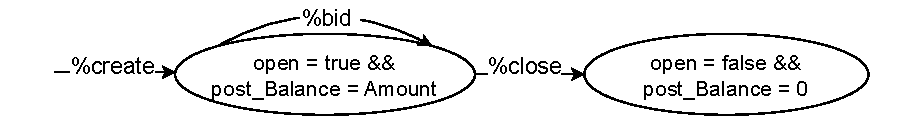
\includegraphics[width=0.9\textwidth]{auction}
    \caption{Auction contract life cycle}
    \label{fig:auction-life-cycle}
\end{figure}

\section{Symbolic Execution Model}
\label{sec:symbolic-execution-model} 
We already learned about Michelson, the low-level smart contract
language for the Tezos blockchain, and its stack-based nature in
Section~\ref{sec:background}.  Here we address the changes needed for symbolic execution of Michelson programs, focusing on a selection of instructions. 
\subsection{System Model}
\label{sec:system-model}
Our symbolic model of a program state consists of a stack where each element is a symbolic value, represented as a pair comprising a Michelson term and its type. Thus, we write a stack as \STACK\ = (\TermOne, \TYF) \STACKCONCAT\ (\TermTwo, \TYS) \STACKCONCAT\ \DOT\ \STACKCONCAT\ \EMPTYSTACK. Here, \ensuremath{[\ ]} represents the empty stack, and \ensuremath{hd :: tl} denotes a stack with \ensuremath{hd} as the top element and \ensuremath{tl} as the remaining stack. Let \INSTRUCTION\ = \InstructionOne; \InstructionTwo; \DOT; \InstructionN\ be a sequence of instructions, and \PREDICATE\ be a path predicate  expressed in conjunctive form, capturing the branching conditions.
\begin{definition}
A symbolic execution state is represented by a tuple \STATE\ =
[\INSTRUCTION, \STACK, \PREDICATE].
A system configuration, \SYSTEM\ = \{\STATEONE, \STATETWO,
\DOT, \STATEN \}, is a set of  states.
\end{definition}
\subsection{Rules}
An instruction is defined by rules on a system configuration. There are two kinds of transitions: (1) \StateTrans\ internal transitions of a state, which are non-deterministic, and (2) \SystemTrans\ system transitions, which pick any state and replace it with all distinct states reachable by internal transitions, exploiting the non-determinism of the \StateTrans\ relation.

A state is unreachable if its predicate \PREDICATE\ is  not
satisfiable. The following rule drops unreachable states.
\begin{mathpar}
\inferrule[]
  { \UNSAT\ \PREDICATE
  }{
  \{[\INSTRUCTION, \STACK, \PREDICATE]\} \cup \SYSTEM \SystemTrans \SYSTEM}
\end{mathpar}
The symbolic interpreter works on a graph with states as nodes and transitions as edges. This representation simplifies performing multi-step sub-transitions needed for some operations.

The semantics of the symbolic rules for the instructions adhere to the formal definition of the Michelson language as outlined in \cite{michelson,michelson1}. In our model, these instructions are classified based on how we handle them into one-step, multi-step, blockchain, cryptographic, branch, and loop instructions. 

One-step instructions directly modify the system state without branching, have a localized effect, and are modeled with a single rule.

Multi-step instructions involve the execution of a sub-sequence of instructions before returning to the main execution. The rule below models the \EXEC\ instruction, which executes a function specified as a sequence of instructions denoted by \INSTRUCTIONONE\ in the rule. This instruction applies the code of the function to the first element of the stack and then places the result back into the main execution.
\begin{mathpar}
  \inferrule[]
  { [\INSTRUCTIONONE, (\StackOne, \TYF) \STACKCONCAT \EMPTYSTACK, 
    \PREDICATE]
    \StateTrans^*
    [ \EMPTYSTACK, (\StackOne', \TYS) \STACKCONCAT \EMPTYSTACK, \PREDICATE']}{[(\EXEC; \INSTRUCTION),   (\{\INSTRUCTIONONE\}, \TYF\ \rightarrow\ \TYS) \STACKCONCAT
    (\StackOne, \TYF) \STACKCONCAT \STACK, \PREDICATE] 
    \StateTrans \
    [ \INSTRUCTION, (\StackOne', \TYS) \STACKCONCAT \STACK,
    \PREDICATE']}
\end{mathpar} 
Here, $\StateTrans^*$ represents the execution of multiple steps in a sequence of internal transitions.

Blockchain instructions, such as the \AMOUNT\
 instruction make implicit use of data from the transaction, the block and the current state of the blockchain. As these values are constant during the execution of a contract, we model them as fixed variables. 

Branch instructions, such as \IF\{\INSTRUCTIONONE\}\{\INSTRUCTIONTWO\} consume a value at the top of the stack. If the branch condition
is True, it executes \INSTRUCTIONONE; otherwise, it executes
\INSTRUCTIONTWO. 
\begin{mathpar}
  \inferrule[]
  { }{
    [(\IF\ \INSTRUCTIONONE\  \INSTRUCTIONTWO; \INSTRUCTION),
    (\StackOne, \TBOOL) \STACKCONCAT\STACK, \PREDICATE]
    \StateTrans\
    \{[\INSTRUCTIONONE; \INSTRUCTION, \STACK, \PREDICATE\ \Wedge\
    \StackOne],   [\INSTRUCTIONTWO; \INSTRUCTION, \STACK, \PREDICATE\ \Wedge\ \NEG\
   \StackOne]\}} 
\end{mathpar}

The loop instructions, including \LOOP\ check the loop condition by examining the
top of the stack. These loop instructions may not terminate, just like while-loops. There are further loop instructions, like \ITER\ and
\MAP, specialized to traverse data structures like lists, sets, and maps. There are also
some instructions that implicitly require looping like \CONCAT, and
\SIZE. The latter kinds of loop instructions do always terminate.

We first look at the terminating loops, such as the \ITER\ instruction, which iterates over a
list. The typing rule for the \ITER\ instruction is as follows: 
\begin{mathpar}
  \inferrule{\JTypeExpr\TEnv{\INSTRUCTION}{\TY \STACKCONCAT \TYA\ \SRightarrow\ \TYA}
  }{
      \JTypeExpr\TEnv{\ITER\ \INSTRUCTION}{\TYLIST\ \TY \STACKCONCAT \TYA\ \SRightarrow\ \TYA}
    }
\end{mathpar}
This rule ensures that if the loop body \INSTRUCTION\ has the type \TY\ \STACKCONCAT\ \TYA\ \SRightarrow\ \TYA, then the entire \ITER\ instruction, when applied to a stack with the top element of type \TY\ \TYLIST\ and the rest of the stack of type \TYA, produces a result stack of type \TYA. 

The following rule handles the  \ITER\ loop for  the non-empty list\footnote{\ITER\ can also iterate over sets and maps, but the details are very similar to the list case and hence omitted.}, while the \ITER\ loop terminates when the list is empty.
\begin{mathpar}
  \inferrule[]
  { \HEAD, \STAIL\ \FRESH \\
    [\INSTRUCTIONONE,  (\HEAD, \TY) \STACKCONCAT\STACK, 
    \PREDICATE]
    \StateTrans^*
    [ \EMPTYSTACK,  \STACK', \PREDICATE']
  }{
    [(\ITER\ \INSTRUCTIONONE ; \INSTRUCTION), (\StackOne, \TYLIST\
    \TY) \STACKCONCAT\STACK, \PREDICATE] \StateTrans \\
    [(\ITER\ \INSTRUCTIONONE ; \INSTRUCTION), (\STAIL, \TYLIST\ \TY)
    \STACKCONCAT\STACK',  \PREDICATE' \Wedge  (\StackOne\
    \EQ\ \{\HEAD; \STAIL \}) ] 
  }
\end{mathpar}
It symbolically executes the instructions \INSTRUCTIONONE\ within the
\ITER\ block with the head of the list (\HEAD) replacing the list. The resulting state transitions to a
new stack (\STACK') and an updated predicate (\PREDICATE' $\Wedge$
(\StackOne\ \EQ\ \{\HEAD; \STAIL\})), where \STAIL\ represents the rest of the list. 

If the list is concrete, the instruction terminates as it simply loops over the elements
of the list. How do we deal with \ITER\ if the list is a symbolic value? One solution could involve running the loop a certain number of times to obtain the symbolic value. However, we can defer that decision by abstracting the result. 

The loop body \INSTRUCTIONONE\ can be considered as a function, say \F,  applied to a stack
of type \TY\ ::\ \TYA, resulting in a stack of type \TYA. 
%\begin{mathpar}
%\Gamma\ \vdash\  \F\ :\ \TY\ ::\ \TYA\ \SRightarrow\ \TYA
%\end{mathpar}
If the first element of
the stack is a list \LIST, and the rest of the stack is \STACKZERO\ =
\StackOne\  \STACKCONCAT\ \StackTwo\ \STACKCONCAT\ ... \STACKCONCAT\
\StackN. Assuming the size of the list \LIST\ is $m$, the \ITER\ {\INSTRUCTIONONE} instruction applies the function \F\ to the stack $m$ times, once for each element of the list \LIST. By unfolding the list once as \{\HEAD; \STAIL\}, the result after 
the first iteration is \STACKONE\ = \StackOneOne\  \STACKCONCAT\
\StackTwoOne\ \STACKCONCAT\ ... \STACKCONCAT\ \StackNOne = \F\ \HEAD\
\STACKZERO, and so on. 

We can represent the value of the stack after running the
instruction \ITER\  as the result of a fold function that applies the
function \F\ to the list. 
\begin{mathpar}
\STACK'\ =  \FOLD\ \F\ \STACKZERO\ \LIST
\end{mathpar}
The \FOLD\ function also can be used to express the result of other loop instructions, such as CONCAT and SIZE, symbolically. 

The similar strategy can be employed for the \MAP\ {\INSTRUCTIONONE} instruction.
\begin{mathpar}
\MAP\ \{\INSTRUCTIONONE\} \Slash\ \LIST\ :: \STACK
\end{mathpar}
The outcome of the \MAP\ \{\INSTRUCTIONONE\} instruction is the result of a map function that applies the function \F\ representing the sequence of instructions \INSTRUCTIONONE\ to the list \LIST. 
\begin{mathpar}
(\FMAP\ \F\ \LIST) ::  \STACK
\end{mathpar}

Finally, we consider a loop instruction that may not terminate, such as \LOOP. 
When the input to the symbolic execution consists of concrete values, an unbounded loop causes the interpreter to iterate for a significant number of times until it halts with an exception indicating an unfinished loop. This mirrors the behavior observed in the actual execution of smart contracts, where the loop continues until it runs out of gas, terminating the computation with an out-of-gas error.

For a symbolic value, the stack type is determined before the loop is executed. We unfold the symbolic value once, execute the loop to determine the operation function, and then abstract the result of the loop and loop condition as function results. This abstraction helps detect whether the loop is unbounded, such as when the abstract function of the loop condition always results  true. 

In separate work \cite{dynamic-logic}, we have designed a dynamic logic tailored to Michelson as a formal foundation for the implementation of SCV. We have formalized a soundness proof of this logic in the Agda proof assistant.
\section{Static Checker}
\label{sec:static-checker-we}
The architecture of the static checker is illustrated in
Figure~\ref{fig:architecture-of-static-checker}. Users write
specifications in the SCV language, which are then parsed into an
Abstract Syntax Tree (AST) in OCaml. The input term along with the
code is passed to the symbolic interpreter, while the output term and
the pre- and postconditions are fed to the static checker. The
symbolic interpreter then runs the code with the provided input, where
the initial stack is derived from the input term.

When a branch occurs, the interpreter sends the path condition to the Z3 converter to convert it into Z3 formulas, which are then passed to the Z3 solver to check whether the path conditions are satisfied. The result of this check determines the interpreter's action; if satisfied, the branch is added, otherwise, it is abandoned. This branch check significantly reduces the number of execution states, especially for stack-based languages like Michelson, where the programmer may need to perform the same check multiple times.

Once the symbolic execution finishes, the results (i.e., all reachable states) are sent to the static checker. Each state contains the post-storage updated after execution, the list of operations to emit, and the path conditions. The static checker then performs the following tasks: output check, property check, and generation of all fail conditions.

We utilize the Z3 library in OCaml to construct the Z3 converter. Some adjustments are necessary to convert these terms into Z3 formulas. For instance, since Z3 does not have a natural number type (\TNAT), it is mapped to Z3's integer type with an additional constraint asserting that the value is greater than or equal to zero. Several constants, such as \CAMOUNT\ and \CBALANCE, as well as cryptographic functions are predefined in the environment that applies to any smart contract specifications.
\begin{figure}[tp]
    \centering
    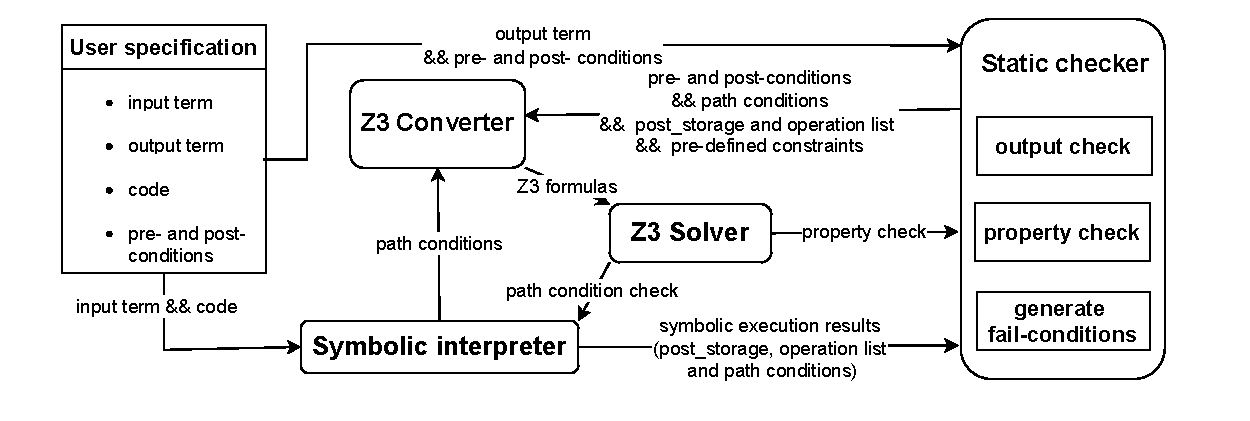
\includegraphics[width=1\textwidth]{scv}
    \caption{The architecture of the static checker}
    \label{fig:architecture-of-static-checker}
\end{figure}

We have implemented approximately 85\% of the Michelson instructions,
including the most frequently used instructions. The remaining instructions were not implemented due to time constraints rather than technical limitations.

Consider the specification of the \lstinline/sub/ contract, the results of
the symbolic execution are either a failwith state with the path
condition \lstinline/x/ $<$ \lstinline/y/,  or a state in which the
final stack has only one element, which is a symbolic variable
\lstinline/sbvar/ of type integer, with the path condition stating
that the variable \lstinline/x/ is greater than or equal to
\lstinline/y/ and  \lstinline/sbvar/ is equal to
the subtract of \lstinline/x/ and \lstinline/y/. 
\subsection{Output check}
\label{sec:output-check}
For a fragment of Michelson code, the output term of the symbolic
execution has the form of a term \Term\ and its type \TY. For a
complete smart contract, it takes the form \PAIR\ \VOPERATIONLIST\
\VSTORAGE, \TPAIR\ (\TOPERATIONLIST) \TYS, where \VOPERATIONLIST\
represents the operation list and \VSTORAGE\ represents
the storage. Given
an output term specified as $\tau$, the checker scans all reachable
final states that do not contain a failwith stack and checks whether
$\tau$ matches the output term. In the former case, it matches
$\tau$ with the term \Term. In the latter case, it matches with
\VSTORAGE.  

For instance, in the \lstinline|sub| contract, the output check ignores the states where the failwith occurs and verifies whether the output term \lstinline|z| matches the symbolic output term \lstinline/sbvar/ in the other state. It succeeds for this example as expected. However, this test could fail if, for example, the output term is incorrectly specified as a variable of a type that does not match the actual result.
\subsection{Fail conditions}
\label{sec:fail-conditions}
A Michelson contract can fail due to conditions introduced by the programmer, triggered by the \FAILWITH\ instruction along with an error message. Failures play a crucial role in smart contract programming to ensure that certain conditions lead to contract termination, such as unauthorized caller attempts (access control properties) or invalid arguments. Various smart contract standards, including \cite{erc,fa}, mandate specific fail conditions.

The static checker includes a feature to generate all fail conditions encountered in a smart contract. SCV identifies all instances where execution terminates due to the \FAILWITH\ instruction, collecting the associated path conditions and error messages. Users receive a comprehensive report detailing each fail condition along with its corresponding message. This capability enables verifying access control properties and other critical aspects across different smart contracts.

For instance, the entrypoint \lstinline|bid| has three fail conditions, as shown in Listing~\ref{lst:fail-condition-auction-contract-bid}: (1) If the auction is closed, (2) if the auction is open but the bid amount is less than or equal to the current balance, and (3) if the auction is open, the bid amount exceeds the balance, but the address of the highest bidder is invalid.
%\lstset{language=michelson}
\begin{lstlisting}[float=tp,captionpos=b,caption={Fail condition for auction contract bid entrypoint},label={lst:fail-condition-auction-contract-bid},numbers=left]
1. not (open = true): 'Already closed'
2. (open = true) && not (Amount > pre_Balance):
   'Not higher than the current highest bid'
3. (open = true) && (Amount > pre_Balance) && 
   get_contract (unit, highest) = None: 'Invalid address' 
\end{lstlisting}
\subsection{Property check}
\label{sec:property-check}
A property is
specified with the clause:  \lstinline/pre-condition := &&/
$\Phi_{i}$ followed by \lstinline/post-condition := &&/ $\Psi_{j}$. This
specification asserts that if all preconditions $\Phi_{i}$ hold before
smart contract execution, then all $\Psi_{j}$ must hold after
successful (i.e., without failure) termination. To verify this
property, the tool explores all the paths $\Pi$ 
with the path condition $\Theta$ such that ($\bigwedge \Phi_{i}$
$\land$ $\Theta$) is satisfiable. It then check that for every path
$\Pi$, $\neg$ ($\bigwedge \Phi_{i}$ $\land$ $\Theta$ $\rightarrow \bigwedge \Psi_{j}$) is unsatisfiable in the context given by the input for the entrypoint
and its final state. For example, for the \lstinline/sub/ contract, the failwith branch is discarded because the precondition does not satisfy the path condition, and then \lstinline/z/ is matched to
the symbolic variable \lstinline/sbvar/ in the other branch. In this
example, the checker finds that $\neg$ ((\lstinline/x/ $>=$ y) $\land$ (\lstinline/z/
= \lstinline/x/ $-$ \lstinline/y/) $\rightarrow$ (\lstinline/z/ $=$ \lstinline/x/ $-$ \lstinline/y/) $\land$ (\lstinline/z/ $>=$ 0)) is unsatisfiable.
\subsection{Life-cycle check}
\label{sec:life-cycle-check}
An entrypoint relation can be defined as \lstinline/(%a -> %b) with
p/, indicating that after invoking the entrypoint \lstinline/%a/, it
is permissible to call the entrypoint \lstinline/%b/ if the condition
\lstinline/p/ holds. The presence of the keyword \lstinline/not/ at
the beginning signals an impossibility. The suffix \lstinline/with p/ may be omitted when no condition is needed.

Let $S_a$ represent the set of all reachable states resulting from the execution of the call to the entrypoint \lstinline/%a/. Each $s_{i}$ in $S_a$ is associated with a path condition $\Theta_i$ and is represented as a stack containing a single element—a pair consisting of an operation list ($\VOPERATIONLIST_i$) and the storage $\VSTORAGE_i$. For each $s_{i}$, symbolic execution is performed on the entrypoint \lstinline/%b/ using input as a pair of the parameter and the storage $\VSTORAGE_i$, constrained by $\Theta_i$ and the condition \lstinline/p/. In the execution state space, a state $s_{j}$ with the path condition $\Theta_j$ is considered reachable if ($\Theta_i$ $\land$ \lstinline/p/ $\land$ $\Theta_j$) is satisfiable, and $\neg$ ($\Theta_i$ $\land$ \lstinline/p/ $\rightarrow$ $\Theta_j$) is unsatisfiable. Let $S_b$ denote the set of these reachable states. If $S_b$ is empty or contains only failwith states, then it is impossible to invoke the entrypoint \lstinline/%b/ from the state $s_{i}$. Otherwise, it is considered a success. Let $R$ be the set containing all such states $s_{i}$ in $S_a$ where it is successful to call the entrypoint \lstinline/%b/ with the condition \lstinline/p/. If $R$ is non-empty, then \lstinline/(%a -> %b) with p/ holds. Otherwise, it is false, signifying \lstinline/not (%a  -> %b) with p/.
\section{Case Studies}
\label{sec:case-stud-subs}
This section reports two case studies which are taken from the realm of financial applications deployed on the Tezos blockchain. 
\subsection{USDtz}
\label{sec:usdtz}
In a blockchain ecosystem, tokens function as digital assets that can be transferred between accounts. These tokens come in various types, which include native tokens (cryptocurrencies) like Bitcoin and Tezos, as well as digital tokens created through smart contracts on an existing blockchain.

It is advisable to implement tokens that adhere to established standards, such as ERC-20 \cite{erc} for Ethereum \cite{eth-whitepaper}, ensuring interoperability and compatibility across different platforms. A token standard specifies a set of rules and an interface that smart contracts must adhere to. The Tezos blockchain has its own set of standards known as Financial Applications (FA) in which FA 1.2 \cite{fa} is designed for fungible tokens.
\begin{lstlisting}[float=tp,captionpos=b,caption={FA 1.2 interface},label={lst:fa12-interface},numbers=left]
pair (address:from, pair (address:to, nat:value)) %transfer
pair (address:spender, nat:value)           %approve
(view pair (address:owner, address:spender) nat) %getAllowance
(view (address:owner) nat)                  %getBalance
(view unit nat)                             %getTotalSupply
\end{lstlisting}

Any contract aiming to implement the FA 1.2 standard must incorporate the functions specified in Listing~\ref{lst:fa12-interface}, where
\lstinline/view a r = pair a (contract r)/ implies an view entrypoint.
A view is an entrypoint that takes an argument of type \lstinline/a/ and a contract to callback that receives in a value of type \lstinline/r/. 
We verify USDtz \cite{usdtzimplemetation,tzstatsusdtz}, an implementation of the FA 1.2 standard. The goal is to ensure that the implementation aligns with the standard, verifying its correctness. USDtz is designed to maintain a stable value by pegging it to a fiat currency like USD or EUR. It has been operational on the Tezos blockchain for a significant time.

The implementation consists of approximately 1000 instructions, covering the five required entrypoints for the FA 1.2 standard and four additional ones. The storage contains a ledger (\lstinline/ledger/), which is a substantial map linking user addresses (\lstinline/user/) to a pair consisting of their balance (\lstinline/balance/) and a map (\lstinline/approvals/) associating addresses (\lstinline/spender/) with the amount of tokens (\lstinline/value/) allowed to be transferred from that user's account. It also includes additional information such as the admin address (\lstinline/admin/), total supply (\lstinline/totalSupply/), and the smart contract state (\lstinline/paused/).

The \lstinline/transfer/ entrypoint credits the account associated with the address provided in the \lstinline/to/ parameter while debiting the account corresponding to the \lstinline/from/ parameter with the specified \lstinline/value/ amount. According to the FA 1.2 standard, this call must fail under two specific conditions: (1) The entrypoint must fail with the error \lstinline/NotEnoughBalance/ if the sender's account lacks sufficient funds. (2) If the sender's account does not have permission to withdraw the specified \lstinline/value/ amount, the call will fail with the \lstinline/NotEnoughAllowance/ error. To verify these requirements, we utilize the failwith condition feature of our tool and examine the returned results, one of which is outlined in Listing~\ref{lst:transfer-udstz-contract-z}. The fail condition results confirm these stipulations.
\begin{lstlisting}[float,captionpos=b,caption={The \lstinline/NotEnoughBalance/ fail condition for the \lstinline/transfer/ entrypoint},label={lst:transfer-udstz-contract-z},numbers=left]
not (paused = true) 
&& get_big_map (from, ledger) = Some sbvar 
&& sbvar = Pair sbvar1 sbvar2 
&& not (sbvar1 >= value) : 'NotEnoughBalance'
\end{lstlisting}

Another essential property is ensuring that the allowance of the sender's account is decremented and the receiver's account is incremented by the \lstinline/value/ that has been sent. This specification is verified to ensure compliance with the contract's intended behavior.

The \texttt{approve} entrypoint grants the spender the right to transfer a specified amount from the owner's account. The contract prohibits changing the allowance value from a non-zero value to another non-zero value to prevent a known attack vector \cite{attack-vector}. This attack exploits the ability to spend the entire allowance before an update and then again after, resulting in a larger amount being spent than allowed. Therefore, the contract call must fail if both the parameter \lstinline/value/ and the current allowance of \lstinline/spender/ are non-zero. We verify this critical property by generating fail conditions to check whenever such a non-zero value update results in a fail condition as Listing \ref{lst:approve-udstz-contract-z}.
\begin{lstlisting}[float=tp,captionpos=b,caption={The non-zero value fail condition for the \lstinline/approve/ entrypoint},label={lst:approve-udstz-contract-z},numbers=left]
not (paused = true) 
&& get_big_map(Sender, ledger) = Some sbvar 
&& sbvar = Pair sbvar1 sbvar2 
&& get_map(spender, sbvar2) = Some sbvar3 
&& not(value = 0) && not(sbvar3 = 0): 'UnsafeAllowanceChange'
\end{lstlisting}

When the update is allowed, the updated value must be correctly recorded in the storage. This can be divided into two sub-properties: (1) if the parameter \lstinline/value/ is zero, then the corresponding allowance value of the \lstinline/spender/ from the owner (which is \SENDER\ in this call) should be zero, and (2) if \lstinline/value/ is non-zero and the allowance of the \lstinline/spender/ is zero, then the \lstinline/value/ should be recorded in the storage after the call. We specify these properties using pre and postconditions, as illustrated in Listing~\ref{lst:specification-approve-p1} for the first property.

The \lstinline/getAllowance/, \lstinline/getBalance/, and \lstinline/getTotalSupply/ entrypoints are view entrypoints that retrieve information from the storage without altering the state of the smart contract. For a view entrypoint implementation, it's crucial to return the \lstinline/TRANSFER_TOKENS/ operation targeted at the specified contract with accurate details. Another important property is that all Tezos tokens passed to a view entrypoint should be forwarded to the callback contract, and there should be no modifications made to the ledger. This ensures that view entrypoints maintain their non-modifying nature, strictly adhering to the expected behavior in blockchain environments.

We specified and verified all the properties mentioned above and others. The results confirm that these properties are guaranteed, ensuring the correctness of the smart contract code.
\begin{lstlisting}[float=tp,captionpos=b,caption={Specification of the \lstinline/approve/ entrypoint (Property 1)},label={lst:specification-approve-p1},numbers=left]
entrpoint %approve
 parameter := Pair (spender: address) (value: nat)
 pre-condition := not (paused = true)
  && get_big_map (Sender, ledger) = 
     Some (v: pair nat (map address nat))
  && v = Pair (n: nat) (m: map address nat) 
  && get_map (spender, m) = Some (k: nat) 
  && not (k = 0) && (value = 0)
 post-condition := get_big_map (Sender, post_ledger) = 
    Some (post_v:  (pair nat (map address nat))
  && post_v = Pair (post_n: nat) (post_m: map address nat) 
  && get_map (spender, post_m) = Some (post_k: nat) 
  && (post_k = 0) ;
\end{lstlisting}
\subsection{Kolibri Oracle Contract}
\label{sec:kolibri-oracle-contr}
The potential of smart contracts is constrained by their inability to access external data sources. To address this limitation, oracles play a pivotal role in providing external data for smart contracts. Since certain essential properties must be satisfied by an oracle contract, including data accountability, this case study illustrates the process of specifying and verifying an oracle contract using SCV, with the Kolibri oracle contract \cite{kolibri} as an example.

The Kolibri oracle contract ensures the accuracy of external data for the Tezos-based stablecoin Kolibri by leveraging the Harbinger Price Feed. The contract initiates calls to a Harbinger Normalizer contract, checks the returned values, normalizes them to suit the Kolibri system, and subsequently relays them to the client. Key attributes stored by the oracle include: the address of the Harbinger contract (\lstinline/harbinger/) \footnote{Here, we shortened the names of the variables for the storage.}, the current state of the contract (\lstinline/state/), a callback contract awaiting Harbinger data (\lstinline/client/), the address of the governor contract (\lstinline/governor/), and the maximum acceptable age of data received from Harbinger (\lstinline/maxDelay/). The oracle contract offers various entrypoints, including:
\begin{itemize}
\item \lstinline/getXtzUsdPrice/: Processes the client request and calls the Harbinger contract.
\item \lstinline/getXtzUsdPrice_callback/: Relays the Harbinger price to the client.
\item \lstinline/setMaxDelaySec/: Resets the \lstinline/maxDelay/ attribute.
\item \lstinline/setGovernorContract/: Allows setting the Governor's address.
\end{itemize}

The Kolibri oracle maintains a state machine with two states: (1) \lstinline/IDLE/ and (2) \lstinline/WAITING_FOR_HARBINGER/. The \lstinline/getXtzUsdPrice/ entrypoint is permissible only when the oracle is in the \lstinline/IDLE/ state; invoking this entrypoint transitions the oracle to the \lstinline/WAITING_FOR_HARBINGER/ state. Conversely, the\\ \lstinline/getXtzUsdPrice_callback/ entrypoint is allowable solely when the oracle is in the \lstinline/WAITING_FOR_HARBINGER/ state; invoking this entrypoint results in the oracle transitioning back to the \lstinline/IDLE/ state. The value of \lstinline/client/ is always set to \lstinline/none/ in the \lstinline/IDLE/ state and to \lstinline/some/ in the other state. We verify this property by examining the fail conditions of these two entrypoints and verifying the entrypoint relations between \lstinline/getXtzUsdPrice/ and \lstinline/getXtzUsdPrice_callback/.

The two subsequent properties dictate that if \lstinline/getXtzUsdPrice/ is successfully executed, the parameters must be stored in the \lstinline/client/ attribute. \\ If \lstinline/getXtzUsdPrice_callback/ is successful, there must be a transaction transferring the data to the client at the \lstinline/client/. These properties are checked by using pre and postconditions. Furthermore, the critical access control property is that the entrypoints \lstinline/setGovernorContract/ and \lstinline/setMaxDelaySec/ must only be invocable by the governor. Any attempts by unauthorized callers to these entrypoints should result in failure.

When verifying the entrypoint \lstinline/setMaxDataDelaySec/, we noticed an unmatched statement. According to \cite{kolibri}, the Kolibri oracle is expected to perform two checks on data returned from Harbinger: (1) confirming the asset returned is 'XTZ-USD' and (2) verifying the asset was updated within the last 30 minutes. We conducted fail condition checks for both the \lstinline/setMaxDelaySec/ and \lstinline/getXtzUsdPrice_callback/ entrypoints, but these conditions were not enforced. Specifically, upon examining the failwith conditions, we detected that there is no failwith when the data is more than 30 minutes (equal to 1800 seconds). 

We then add the predicate \lstinline/post_maxDelay <= 1800/ in the postcondition of the entrypoint \lstinline/setMaxDataDelaySec/ as shown in Listing \ref{lst:setMaxDataDelaySec1}, but then the pre and postcondition test fails. This means there is no constraint enforcing that the data must be less than or equal to 30 minutes. This constraint is possibly set up by the governor and specified in the \lstinline/MaxDataDelaySec/ field. However, users calling this contract should be aware that it is possible for the governor to set any value ($>=0$) as desired. This could lead to providing out-of-date rates.
\begin{lstlisting}[float=tp,captionpos=b,caption={The specification of the \lstinline/setMaxDataDelaySec/ entrypoint},label={lst:setMaxDataDelaySec1},numbers=left]
entrypoint %setMaxDataDelaySec
 code := {...}
 parameter := delay: nat
 pre-condition := Sender = governor            
 post-condition := post_harbinger = harbinger 
 && post_governor = gover
 && post_maxDelay = delay && post_maxDelay <= 1800
\end{lstlisting}

The complete specifications and experimental results for the examples and case studies can be accessed online at \cite{scv}.
\section{Related Work}
\label{sec:related-work}
In this section, we discuss some key approaches, particularly those employing symbolic execution in the context of smart contracts. P. Tsankov et al. introduced
SECURIFY \cite{securify}, a tool that utilizes symbolic execution to
perform practical security analysis on Ethereum smart contracts. It
targets common vulnerability security patterns specified in a
designated domain-specific language. 
Similarly, Manticore
\cite{manticore} and KEVM \cite{kevm} also target Ethereum smart contracts. KEVM is an executable formal
specification built with the K Framework.
Since tokens can hold a significant amount of value, they are often targeted for
attacks. Therefore, several tools \cite{kevm,park} conduct case
studies for the implementations of token standards. 

Several approaches use existing formal verification frameworks to
ensure the correctness and security of smart contracts. S. Amani et
al. \cite{isabelle} proposed the formal verification of Ethereum smart
contracts in Isabelle/HOL. Hirai \cite{hirai} formalizes the EVM using
Lem, a language to specify semantic definitions. 

There are existing tools for automated verification include solc-verify \cite{solc}, VerX \cite{verx}, and Oyente \cite{oyente}. solc-verify processes smart contracts written in Solidity and discharges verification conditions using modular program analysis and SMT solvers.
While these approaches differ, they share a focus on common bugs (such as reentrancy, overflow or underflow, and frozen funds). Our tool provide an environment where users can reliably specify their own properties and identify contract-specific bugs. Our tool aims to rich specifications to supports manually specified full correctness specifications.

Close to our approach are HELMHOLTZ \cite{helmholtz} and Mi-Cho-Coq \cite{micho}, as discussed in Section \ref{sec:introduction}. In HELMHOLTZ, properties are annotated inside the code by the developer, which requires modifying the code. In contrast, we provide a separate specification language, so users do not need to modify the code. Similar to our tool, iContract \cite{icontract} utilizes symbolic execution and pre and postconditions to specify user properties, but the iContract work and our work differ in target language, DSL design, and functionality.
\section{Conclusion}
\label{sec:concl-sect-append}
Symbolic execution is well known to suffer from challenges related to state explosion, particularly when applied to large systems. To address this problem, our tool mitigates state explosion and has been applied to two real case studies of running blockchain contracts, focusing on significant subjects such as token standards and oracles.

Our tool has several limitations. SCV relies on Z3, which may struggle with very large or complex problems, potentially returning \texttt{unknown} if it cannot determine satisfiability. Additionally, the tool does not yet handle gas consumption or support external calls.
In future work, we want to extend SCV in two directions. 
First, we want to address the interaction of several entrypoints by
extending the specification language to state allowed sequences of
contract invocations.  Second, a Michelson program returns a list of instructions, which may contain
further contract invocations. Dealing with this kind of contracts
requires an extension to the symbolic interpreter so that a sequence
of contract invocations can be processed in one run.
\newpage
\bibliographystyle{splncs04}
\bibliography{bio}
%\newpage
%\appendix
\chapter{Assertion Grammar in EBNF}\label{apx:grammar}
The following two versions of the grammar implement the prefix and infix notations for the assertion syntax. 
\todo{Rename mutez}

\section{Prefix notation}
\lstinputlisting[basicstyle=\linespread{1.0}\fontfamily{lmr}\selectfont\small,
				 backgroundcolor=\color{cverbbg},
				 linewidth=14cm,
				 xleftmargin=0.5cm,
				 frame=lr,
				 framesep=8pt,
				 framerule=0pt,
				 captionpos=b,
				 numbers=none,
				 language=,
				 caption=Assertion grammar with prefix notation]{../grammar/assertion_grammar_prefix.txt}

\section{Infix notation}
\lstinputlisting[basicstyle=\linespread{1.0}\fontfamily{lmr}\selectfont\small,
				 backgroundcolor=\color{cverbbg},
				 linewidth=14cm,
				 xleftmargin=0.5cm,
				 frame=lr,
				 framesep=8pt,
				 framerule=0pt,
				 captionpos=b,
				 numbers=none,
				 language=,
				 caption=Assertion grammar with infix notation]{../grammar/assertion_grammar_infix.txt}

\chapter{List accessing in Michelson}\label{apx:nth}

\lstinputlisting[basicstyle=\linespread{1.0}\fontfamily{lmr}\selectfont\small,
				 backgroundcolor=\color{cverbbg},
				 linewidth=14cm,
				 xleftmargin=0.5cm,
				 frame=lr,
				 framesep=8pt,
				 framerule=0pt,
				 captionpos=b,
				 numbers=none,
				 language=,
				 label=lst:nth_liq,
				 caption=Possible implementation of \texttt{nth} in Liquidity]{listings/nth.liq}
				 
\lstinputlisting[basicstyle=\linespread{1.0}\fontfamily{lmr}\selectfont\small,
				 backgroundcolor=\color{cverbbg},
				 linewidth=14cm,
				 xleftmargin=0.5cm,
				 frame=lr,
				 framesep=8pt,
				 framerule=0pt,
				 captionpos=b,
				 numbers=none,
				 language=,
				 label=lst:nth_tz,
				 caption=\lstref{lst:nth_liq} compiled to Michelson]{listings/nth.tz}
\end{document}

